\chapter{Introduction} \label{introduction} \todo{process comment Hans: Work towards an
introduction that explains the problem question in the Research question section. Add
motivation, passion for the subject and experience, and relate this to NS.}

\enquote{\emph{Pantha Rhei}} is, according to \emph{Plato}, one of the famous
philosophical statements first described by the Greek philosopher
\emph{Heraclitus}\footnote{\url{https://plato.stanford.edu/entries/process-philosophy/}}.
Translated as \enquote{everything flows} this statement is an unambiguous commitment to
the ubiquitous dynamics of everything that exists. \enquote{Life is flux}, one of the
constants in life, is change.

In the realms of Software Engineering, the \enquote{laws of software evolution}
\parencite[]{lehman_programs_1980} refers to a series of laws described by
\citeauthor{lehman_programs_1980}. With these Laws, he describes the balance between the
forces driving new developments on the one hand (a change) and the forces that slow down
progress on the other hand. Based on \emph{Heraclitus} philosophical statement, this paper
assumes that software engineering projects will frequently be subjected to change,
probably due to changing market demands or technological progress. 

More than a half of century of software engineering-, and architecture practices show that
the complexity of these software artifacts gradually increases over time. Eventually, this
will render most of the software artifacts obsolete, according to
\citeauthor{lehman_programs_1980} \parencite[]{lehman_programs_1980}.

We also observe that contemporary competitive corporate environments are changing
continuously. The speed at which these changes emerge is also increasing. To stay
competitive it is essential to be able to deal with corporate change and shifting market
demands. \todo{add a citation to the work of Steven de Haes}This is partly driven by
contemporary digital transformations. (IT) Organizations are attempting to cope with this
trend by adopting agility and maturing their agile practices
\parencite[]{2024_SIM_key_issues_and_trends}. Therefore, agility has been proposed as a
measure for contemporary organizations to adapt to new environments and cope with rapid
change \parencite[]{neumann_strategic_1994}.

Over the years, a lot of research is done to mitigate the risks of software artifact
degradation over time. There is also plenty of experience described in various books from
corporate experience. Two of these are part of this research are the Theorems of
Normalized Systems and Uncle Bob's Clean architecture.



\section{Introduction on Normalized Systems} \label{sec:inro_ns}

The Normalized Systems theorems are a scientific approach to creating software systems
based on the laws for software evolvability. These theorems have resulted in a documented
track record of achieving software stability, in a scientific environment. Effectively, it
prevents the accumulation of combinatorial effects on anticipated change drivers. This
prevents the positive feedback loop and prevents the degradation of the software artifact.
Preventing positive feedback loops has a positive effect on the evolvability of software
artifacts.\parencite[]{mannaert_normalized_2009}. 

\citeauthor[]{mannaert_normalized_2009} have formulated the theorem of Normalized Systems
as prescriptive structures (elements) that lead to a modular architecture with low
coupling and high cohesion. The resulting software architecture will be designed to cope
with future change \parencites[]{mannaert_normalized_2009}.
\section{Introduction to Clean Architecture} \label{sec_into_ca}

\ca is the accumulation of more than half a century of coding, designing, and
architecting software systems by \citeauthor*[]{robert_c_martin_clean_2018}. He published
his experience in his book \citetitle*[]{robert_c_martin_clean_2018} in
\citeyear[]{robert_c_martin_clean_2018}. In this book, he states that creating a software
artifact requires less skill and knowledge. However, creating stable and evolvable
software artifacts is a skill that requires a lot of knowledge, skill, dedication, and
time.

The book aims for a software architecture that minimizes the human resources required to
build and maintain the information system. Like \ns, it has a
prescribed design of software classes that will lead to a modular architecture with low
coupling and high cohesion \parencite{robert_c_martin_clean_2018}.

\section{Introducing Software evolvability}
the effort to apply change should stay constant over time, regardless of the type of change,
whether it would be a functional, technical or architectural change.

<<To-do: Link software evolvability to the first part of the introduction>>\\
<<To-do: Link combinatorial effects to a measure to determine software evolvability>>
\newpage \section{Research relevance} \label{research_relevance} 

<<UNDER CONSTRUCTION>>

Since the introduction of Normalized Systems Theorems, Java EE (Java Enterprise Edition)
has been the prevalent programming language used in scientific research settings. It has
been used to describe the evolvability of software architectures based on the stability
concepts of systems theory \parencite[]{mannaert_towards_2012}.

\citeauthor{mannaert_towards_2012} stated in the paper that the design theorems were
formulated as modular structures that are independent of any software language or
development paradigm. The applicability of Normalized Systems Theorems with

Java EE is still a prevalent programming language for enterprise- and IT organizations.
Many software solutions are created and maintained using this programming language.
\section{Hypothesis} \label{hypothesis} 

The proposed hypothesis is that both 'Clean Architecture' and 'Normalized Systems' lead
to a modular software architecture with reduced combinatorial effects. Consequently, both
architectural approaches will lead to improved stability and evolvability of the
Information system.

Both architectural approaches formulate their modular structures independent of any
given programming technology \parencite[]{mannaert_normalized_2009,martin_clean_2018}. As
such, improvements in terms of stability and evolvability are equally applicable for the
C\# artifact used in this research, compared to case studies where Java SE has been used.
\parencites[]{oorts_building_2014, de_bruyn_enabling_2018}.

\begin{figure}[!ht]
    \centering
    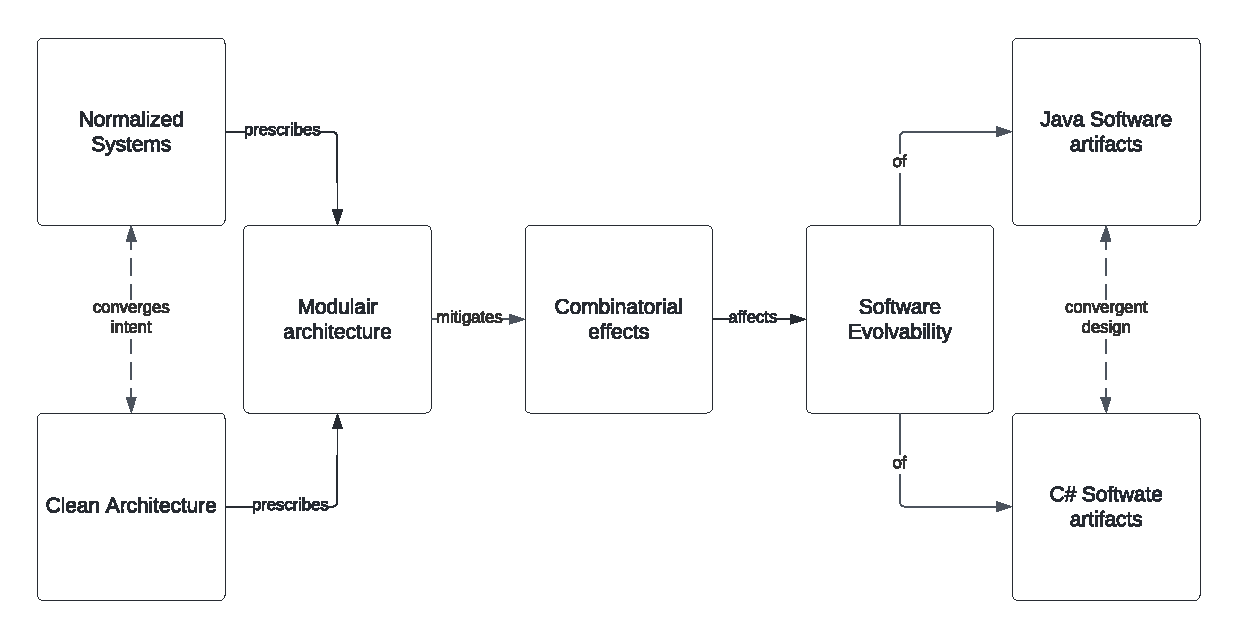
\includegraphics[width=0.9\textwidth]{Figures/hypothesis.pdf}
    \caption[The hypothesis]{The hypothesis}
    \label{fig_hypothesis}
\end{figure}
\section{Research questions} \label{research_questions}
The Hypothesis described in \ref{hypothesis} and \ref{conceptualframework} leads us to the
following research question:

\begin{center}
    \enquote*{\textit{To what extent converges the evolvability of a C\# artifact built
    based on the Clean Architecture principles towards a similar artifact that is based on
    Normalized Systems Theorems?}}
\end{center}

The following sub-questions can be formulated that support the research on the main
research question:
\begin{itemize}
    \item How does Clean Architecture contribute to Software Evolvability?
    \item To what extent Is Normalized Systems applicable to a C\# artifact?   
\end{itemize}
\section{Research model} \label{research_model}

Figure \ref{fig_conceptual_framework} depicts the overall conceptual research framework.
The artifact is the research context. It is a fully functional commerce Restful API with
ASP.NET (v6) and C\# (v10). The research aims to test the cause-and-effect relationship
between Clean Architecture (independent variable) and the evolvability of the C\#
artifact.

The Normalized Systems Theorems do not affect Clean Architecture as an independent
variable. Instead, it will affect the design of the artifact. Previous research and case
studies have already shown that Normalized Systems affect the evolvability of software
artifacts by using a prescribed modular design, mitigating combinatorial effects.
Normalized Systems Theorems is the control variable in the conceptual framework.

Since we are trying to prove the convergence of Normalized Systems and Clean
Architecture the Modular architecture will be compared with the design of Normalized
Systems. Therefore, Modular Architecture is positioned as the Mediator variable in this
conceptual framework.

\begin{figure}[!ht]
    \centering
    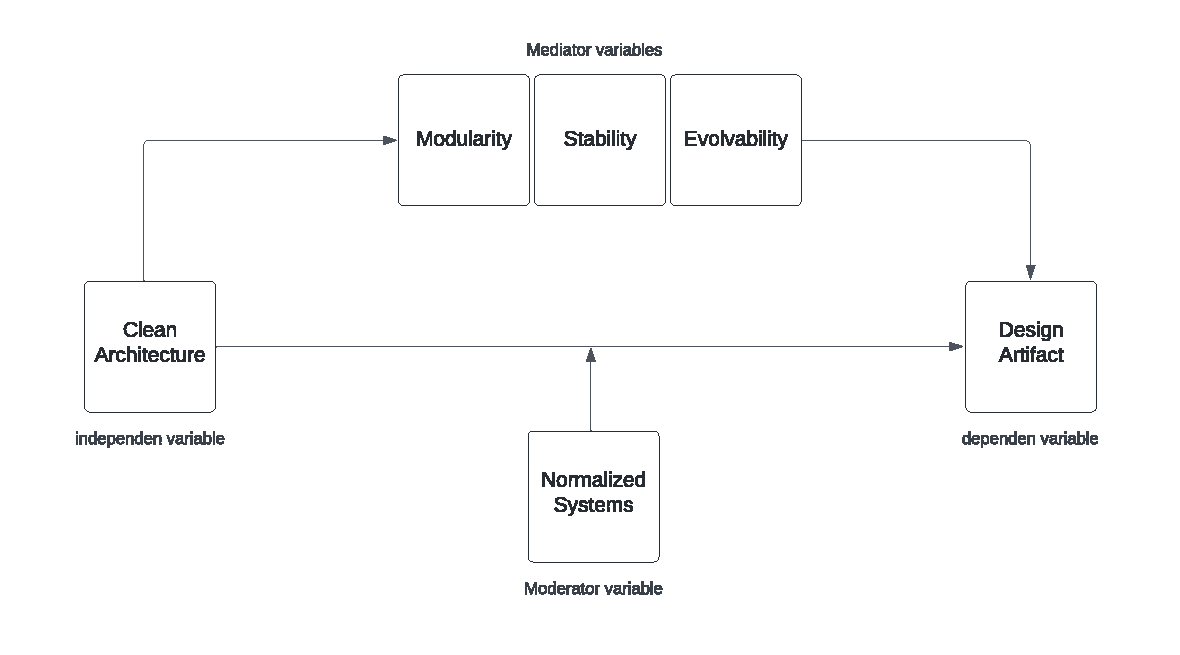
\includegraphics[width=1\textwidth]{Figures/conceptual_framework}
    \caption[Overall conceptual framework]{Overall conceptual framework}
    \label{fig_conceptual_framework}
\end{figure}
